\title{Supplementary material}
\author{\begin{minipage}{0.94\textwidth}\centering
\normalsize Mingyang Li\textsuperscript{1}, Jiabei Liu\textsuperscript{2,*}, Jiayue Gao\textsuperscript{2}\\[6pt]
\small \textsuperscript{1}Beijing Institute of Technology, Beijing, China\\[3pt]
\textsuperscript{2}Jinan University--University of Birmingham Joint Institute,\\
Jinan University, Guangzhou, China\\[6pt]
\textsuperscript{*}Corresponding author: Jiabei Liu\\
\href{mailto:jxl2043@student.bham.ac.uk}{\texttt{jxl2043@student.bham.ac.uk}}
\end{minipage}}
\date{2 November 2026}
\maketitle
\section*{Model selection and performance estimation can diverge: a RoadSens-4M audit and a nine-acquisition PVS case study}
Working version 13, 2 November 2026. This supplement accompanies \path{main_body.tex}. All tables refer to completed canonical runs unless expressly labelled exploratory. The RoadSens main tables report five-fold arithmetic means; PVS tables specify three outer-domain means or individual domains; tables explicitly labelled pooled OOF use the combined heldout predictions. Computational fit-fold counts are not independent scientific sample sizes. The original 1,580-fit suite and targeted post-draft extensions are reported separately.

\section*{S1. Execution matrix and evidence index}
\begingroup\small\setlength{\tabcolsep}{3.5pt}\renewcommand{\arraystretch}{1.14}
\begin{tabularx}{\linewidth}{XYYY}
\toprule
Block & \makecell[r]{Fixed\\ comparison} & \makecell[r]{New\\ canonical\\ fit-folds} & \makecell[r]{Authoritative\\ output} \\
\midrule
A & Four models × four feature sets × three splits × two policies × five folds; seed 42 & 480 & \path{../runs/main_A_v2/analysis/main_A_analysis.md} \\
R & RF seeds 43/44 × four features × random/recording × two policies × five folds & 160 & \path{../runs/consistent_runtime_R_v1/}; \path{../runs/auxiliary_summary_v1.md} \\
B & Three non-RF models × full/context × random/recording × two policies × seeds 43/44 × five folds & 240 & \path{../runs/phase_B_v1/}; \path{../runs/auxiliary_summary_v1.md} \\
C & RF × eight ablations × three splits × two policies × five folds & 240 & \path{../runs/phase_C_v2/independent_validation.md} \\
D & Three additional capacity/budget combinations × three splits × two policies × five folds & 90 & \path{../runs/phase_D_capacity_vs_A_v1.md} \\
E & Binary RF × four feature sets × three splits × five folds & 60 & \path{../runs/phase_E_v1/}; \path{../runs/auxiliary_summary_v1.md} \\
H & Specified component-heldout H1 (100) and byte-copy-removal H2 (90) fits & 190 & \path{../runs/content_overlap_v2/analysis/} \\
I & Two spatial grids × two models × three feature groups × five folds & 60 & \path{../runs/spatial_binary_v1/independent_summary.md} \\
S & STRIDE: two models × two feature sets × three seeds × five folds & 60 & \path{../runs/stride_supplement_v2/validation_summary.md} \\
Total & Includes120 A RF reproduction fits; excludes330 earlier exploratory fits & \textbf{1,580} & \path{../execution_inventory.json} \\
\bottomrule
\end{tabularx}
\endgroup
All canonical blocks completed without a recorded fit failure and underwent independent source/prediction/metric checks. The shared environment is Python3.13.12, scikit-learn1.9.0, NumPy2.5.2, pandas3.0.5, joblib1.5.3, SciPy1.18.0, and threadpoolctl3.6.0. These CPU experiments use at most four threads per fit; a GPU is not required. Hardware timings are not controlled algorithmic speed comparisons.

The immutable cache hash is \path{fa2078df1857f7872c13c6fe187f0883d85a23f9d15fdb3c6897a53314fdea16}. The parent pilot, shared runner, auxiliary driver, source archives, exact split maps, preflights, and model hashes are separately indexed in the execution inventory. Read \path{../reproducibility notes} for commands rather than reconstructing splits from seed values.

\section*{S2. Contribution and prior-work boundary}
\begingroup\small\setlength{\tabcolsep}{3.5pt}\renewcommand{\arraystretch}{1.14}
\begin{tabularx}{\linewidth}{XYYY}
\toprule
Topic & \makecell[r]{Established\\ or\\ closest\\ source} & \makecell[r]{Specific\\ evidence\\ added\\ here} & \makecell[r]{Claim\\ excluded} \\
\midrule
Smartphone road classification & RoadSens data descriptor and archive; CKDP-PINNFed & A fixed v3 payload reconstructed into explicit cohorts and comparable fit/test membership & A first RoadSens classifier or exact replication of the source baseline \\
Contextual/GPS information & RoadSens source fields; CKDP-PINNFed coordinate processing & GPS/availability/context controls under two declared blank-label policies & First GPS use; GPS is always harmful; mask performance proves causal leakage \\
Structured evaluation & Roberts et al.; Ploton et al. & File, content-component, and buffered spatial diagnostics on this snapshot & A new cross-validation algorithm or a verified independent-road benchmark \\
Data redundancy & This version's exact file and finite-axis audit & A byte-identical pair and three exact-content connected groups, with non-monotone predictive changes after regrouping & All score inflation is caused by duplicates; matching content proves route identity \\
Separate-source data & STRIDE descriptor and v4 archive & Seventeen offline recording-type examples with duration controls & Full three-class external validation, transfer, or new-device generalization \\
\bottomrule
\end{tabularx}
\endgroup
The Chinese contribution matrix supplies more detailed claim-to-evidence links. The reference-verification note distinguishes source statements from locally observed results and records access limitations. This is a bounded review, not a priority certificate.

\section*{S3. Same-runtime RF seed checks}
\setcounter{table}{0}
\begin{minipage}{\linewidth}
\captionof{table}{Full-numeric random-minus-recording differences of five-fold mean macro-F1.}
\begingroup\small\setlength{\tabcolsep}{3.5pt}\renewcommand{\arraystretch}{1.14}
\begin{tabularx}{\linewidth}{XYYY}
\toprule
Policy & Seed 42 & Seed 43 & Seed 44 \\
\midrule
Primary & 0.5656 & 0.5387 & 0.5354 \\
Blank-as-normal & 0.5360 & 0.5548 & 0.5148 \\
\bottomrule
\end{tabularx}
\endgroup
\end{minipage}
Each of the five fold-index differences has the same positive direction within every seed/policy configuration. Fold numbers from different splitting schemes do not represent matched independent roads; no paired-road significance test is inferred. Additional full/context model results for all specified B configurations, including weaker logistic-regression patterns, appear in the final auxiliary summary. No best seed or feature combination is selected for the primary table.

Historical seed 43/44 serialized RF estimators used sklearn1.5.2, while seed 42 used1.9.0. They remain historical evidence; R refits the frozen source/row partitions under1.9.0 and supplies the same-runtime comparison above. Original source-level assignments are preserved because regenerating a stratified group partition under a different library version need not reproduce it.

\section*{S4. All main conditional uncertainty contrasts}
All estimates below are \textbf{pooled OOF macro-F1 differences}, not fold-mean differences. Components, strata, and the 2,000 shared weight vectors are frozen. Intervals use the 2.5th and 97.5th empirical percentiles and retain fixed fitted predictors. Every listed contrast has2,000/2,000 valid draws. Strata contain only five normal-only components and 91 mixed components; these intervals cannot establish a general road/device population or training uncertainty.

\setcounter{table}{1}
\begin{minipage}{\linewidth}
\captionof{table}{Twenty-four specified main-model contrasts.}
\begingroup\small\setlength{\tabcolsep}{3pt}\renewcommand{\arraystretch}{1.12}
\begin{longtable}{L{0.148\linewidth}R{0.188\linewidth}R{0.237\linewidth}R{0.079\linewidth}R{0.227\linewidth}}
\toprule
Policy & Model & Contrast & Estimate & \makecell[r]{Conditional95\%\\ interval} \\
\midrule
\endfirsthead
\toprule
Policy & Model & Contrast & Estimate & \makecell[r]{Conditional95\%\\ interval} \\
\midrule
\endhead
Primary & RF100 & Full random − recording & +0.5827 & [+0.4363,+0.6960] \\
Primary & RF100 & Full random − temporal & +0.1798 & [+0.1284,+0.2398] \\
Primary & RF100 & Recording context − full & +0.1853 & [+0.0812,+0.3154] \\
Primary & Extra Trees & Full random − recording & +0.5480 & [+0.3917,+0.6679] \\
Primary & Extra Trees & Full random − temporal & +0.1973 & [+0.1411,+0.2593] \\
Primary & Extra Trees & Recording context − full & +0.0047 & [−0.1596,+0.1781] \\
Primary & HistGB & Full random − recording & +0.5249 & [+0.3928,+0.6350] \\
Primary & HistGB & Full random − temporal & +0.1490 & [+0.1099,+0.1991] \\
Primary & HistGB & Recording context − full & +0.1015 & [−0.0648,+0.3390] \\
Primary & Logistic regression & Full random − recording & +0.3411 & [+0.2129,+0.4169] \\
Primary & Logistic regression & Full random − temporal & +0.0424 & [+0.0186,+0.0690] \\
Primary & Logistic regression & Recording context − full & −0.1297 & [−0.2353,−0.0596] \\
Blank-as-normal & RF100 & Full random − recording & +0.5455 & [+0.4881,+0.6042] \\
Blank-as-normal & RF100 & Full random − temporal & +0.3496 & [+0.2820,+0.4257] \\
Blank-as-normal & RF100 & Recording context − full & −0.0364 & [−0.0893,+0.0164] \\
Blank-as-normal & Extra Trees & Full random − recording & +0.4760 & [+0.4232,+0.5338] \\
Blank-as-normal & Extra Trees & Full random − temporal & +0.3346 & [+0.2712,+0.4002] \\
Blank-as-normal & Extra Trees & Recording context − full & −0.0360 & [−0.0809,+0.0072] \\
Blank-as-normal & HistGB & Full random − recording & +0.5303 & [+0.4666,+0.5905] \\
Blank-as-normal & HistGB & Full random − temporal & +0.3107 & [+0.2575,+0.3718] \\
Blank-as-normal & HistGB & Recording context − full & +0.0247 & [−0.0119,+0.0666] \\
Blank-as-normal & Logistic regression & Full random − recording & +0.1197 & [+0.0578,+0.1822] \\
Blank-as-normal & Logistic regression & Full random − temporal & +0.0444 & [+0.0241,+0.0644] \\
Blank-as-normal & Logistic regression & Recording context − full & −0.0382 & [−0.0852,+0.0071] \\
\bottomrule
\end{longtable}
\endgroup
\end{minipage}
\setcounter{table}{2}
\begin{minipage}{\linewidth}
\captionof{table}{Additional paired RF ablations using the same draws.}
\begingroup\small\setlength{\tabcolsep}{3.5pt}\renewcommand{\arraystretch}{1.14}
\begin{tabularx}{\linewidth}{XYYY}
\toprule
Policy & Contrast & Estimate & \makecell[r]{Conditional95\%\\ interval} \\
\midrule
Primary & Recording numeric-minus-context − full & −0.1179 & [−0.2486,−0.0208] \\
Blank-as-normal & Recording numeric-minus-context − full & −0.0610 & [−0.1064,−0.0185] \\
\bottomrule
\end{tabularx}
\endgroup
\end{minipage}
The prediction row IDs, truths, and stored estimator class order are aligned before comparing A with C. The C validation file stores these paired results; the main A bootstrap directory stores component confusions, draws, and provenance hashes. These are predictive comparisons after fitting different feature representations, not causal interventions on acquisition context.

\section*{S5. Content-component and byte-copy-removal designs}
H1 uses the same 101-source supervised cohort as the main analysis. Seed 42 fits RF100 and HistGB with full/context/IMU features under both policies (60 fit-folds). Seeds 43/44 fit RF100 with full/context features under both policies on their own component-heldout maps (40). Total H1 is 100. H2 excludes source 47 by the label-blind duplicate-file rule and fits RF100 for full/context/IMU, random/recording/temporal, both policies (90). Both H1 and H2 preserve their complete frozen cohorts and report every specified configuration.

For H1 seed 42 versus main recording holdout, twelve same-cohort pooled comparisons comprise six increases and six decreases. The range approximately−0.0462 to+0.0340 is not a duplicate-effect confidence interval. Group changes alter training/testing composition. H2 removes only a byte copy and leaves the partial inertial overlaps; it should not be labelled completely deduplicated.

\setcounter{table}{3}
\begin{minipage}{\linewidth}
\captionof{table}{H2 RF full-feature pooled OOF macro-F1, rounded to three decimals.}
\begingroup\small\setlength{\tabcolsep}{3.5pt}\renewcommand{\arraystretch}{1.14}
\begin{tabularx}{\linewidth}{XYYYY}
\toprule
Policy & \makecell[r]{Cohort\\ supervised\\ rows} & Random & Temporal & Recording \\
\midrule
Primary & 32,838 & 0.995 & 0.818 & 0.445 \\
Blank-as-normal & 61,484 & 0.931 & 0.583 & 0.391 \\
\bottomrule
\end{tabularx}
\endgroup
\end{minipage}
These values are not paired effects against the 101-file main table. Ten policy/fold H2 time-block membership checks verify retention of the original inclusive one-second embargo. The H independent analysis checks all 190 model hashes and 1,795,048 heldout prediction rows across configurations; this prediction-row count repeatedly includes the same underlying observations and is not a sample-size claim.

\section*{S6. STRIDE recording-level supplement}
\setcounter{table}{4}
\begin{minipage}{\linewidth}
\captionof{table}{Pooled OOF macro-F1 across the same 17 STRIDE observations.}
\begingroup\small\setlength{\tabcolsep}{3.5pt}\renewcommand{\arraystretch}{1.14}
\begin{tabularx}{\linewidth}{XYYYY}
\toprule
Features & Model & Seed 42 & Seed 43 & Seed 44 \\
\midrule
Ten sensor norm summaries & RF100 & 0.7639 & 0.8235 & 0.8235 \\
Ten sensor norm summaries & Scaled logistic regression & 0.7639 & 0.8786 & 0.8211 \\
Duration only & RF100 & 0.5882 & 0.5278 & 0.4706 \\
Duration only & Scaled logistic regression & 0.3561 & 0.4396 & 0.3529 \\
\bottomrule
\end{tabularx}
\endgroup
\end{minipage}
The two sensor streams are summarized separately; asynchronous timestamps are not interpolated into invented event windows. A recording folder provides one whole-record type label. Duration is deliberately separated from sensor summaries. Small and stratified test folds, a single device identifier, lack of Normal labels, and unverified physical-route independence prevent deployment or external-three-class conclusions.

The official v4 ZIP has SHA-256 \path{475853a7aaf9a15068dc9c17014f3e46197acc4b705cd3851b84692cdd82f851}. The official source record reports CC BY4.0; author attribution and any applicable third-party requirements still belong in a public release plan. No original data are publicly redistributed by this working manuscript.

\section*{S7. Exploratory temporal controls and annotation runs}
Before the expansion, RF primary/sensitivity recording-heldout macro-F1 for a raw-axis one-second statistics control was0.3953/0.3972. The twenty-dimensional physical one-second representation scored0.3751/0.3759, and its prefix-calibrated variant0.4015/0.3706. These historical scores informed closing the proposed physical-representation branch. However, targeted runtime verification subsequently identifies sklearn1.5.2 in the historical raw-axis control, whereas the main baseline environment is 1.9.0. The old comparison is therefore cross-version exploratory evidence, not a controlled same-runtime representation ranking. New same-runtime window results must determine any updated claim; no new physical-method contribution is inferred from the old scores. These fits are not additional canonical expansion fits.

The raw-axis control has60 dimensions versus20 for the physical representation. These different capacities do not prove one is inferior in all settings. Rolling windows calculated before row splitting can also share raw signal context across heldout rows. Consequently, temporal-feature random-row results are not independent-window evidence. Main expansion features are instantaneous per-row representations and are not described as event or sequence models.

The 348 continuous labelled runs are149 Pothole plus199 Bump runs. All have sampled rows. Secondary equal-run-weight row agreement and majority-label correctness describe these observed segments; neither validates physical boundaries, new-event recall, localization delay, or false alarms per hour. Details remain in \path{../annotated_runs_README.md} and the accompanying machine-readable run summaries.

\section*{S8. Retained failures, revisions, and publication boundary}
Main\_A\_v1 stopped at an RF reproduction mismatch under the unintended sklearn1.5.2 interpreter. Its diagnostic and failed attempt are retained. A correct-runtime diagnostic reproduces6,577/6,577 labels for the checked first fold, and all 120 main A RF reproduction folds subsequently pass. STRIDE\_v1 failed before fitting because of a manifest NameError; v2 is canonical. The unexecuted first H implementation omitted the temporal embargo and was corrected before H\_v2 fitting. Earlier content-map drafts, checks and version-specific corrections are retained. C\_v1 was interrupted during scheduler handoff; full C\_v2 is canonical and the partial run is excluded from the total.

These revisions do not represent score-based selection of favourable fits. Incorrect/partial versions do not fill planned matrix cells. The reproducibility guide identifies commands and authoritative outputs. The public code, protocols, compact evidence and manuscript are available at \url{https://github.com/Asuna-art/roadsens-evaluation-audit}. The initial public code snapshot is commit \texttt{66eb1995a61460c866581122fa86ea908d08b640}. Public views omit signal matrices, direct label/prediction arrays and coordinates and do not replace complete historical inputs. Raw data and model binaries are excluded. The repository README states the environment and replay limitations; author-contribution and venue-specific declarations still require completion.

\section*{S9. Targeted anchor-stride sensitivity}
The frozen post-draft design is recorded in \path{../key_experiments/protocol_key_v1.md}. Only strides 5 and 20 add new RF100 fits; stride 10 is the original A reference. Both label policies, full/IMU features and the original filename fold mapping are retained. New stride populations are reconstructed from full-cadence arrays and live raw annotations. Before fitting, reconstruction at stride 10 matches the cached full/IMU feature values, ordered labels and source identities, and all original fit/test sequences. All 101 source files match their frozen hashes.

\setcounter{table}{5}
\begin{minipage}{\linewidth}
\captionof{table}{All eight new sampling configurations; recording-heldout seed 42, RF100.}
\begingroup\small\setlength{\tabcolsep}{3.5pt}\renewcommand{\arraystretch}{1.14}
\begin{tabularx}{\linewidth}{XYYYYY}
\toprule
Stride & Policy & Features & Rows & \makecell[r]{Fold\\ mean\\ macro-F1} & \makecell[r]{Pooled\\ OOF\\ macro-F1} \\
\midrule
5 & Primary & Full numeric & 65,774 & 0.4386 & 0.4323 \\
5 & Primary & IMU12 & 65,774 & 0.3379 & 0.3408 \\
5 & Blank-as-normal & Full numeric & 123,411 & 0.3866 & 0.3726 \\
5 & Blank-as-normal & IMU12 & 123,411 & 0.3432 & 0.3402 \\
20 & Primary & Full numeric & 16,440 & 0.4086 & 0.4049 \\
20 & Primary & IMU12 & 16,440 & 0.3386 & 0.3400 \\
20 & Blank-as-normal & Full numeric & 30,889 & 0.3765 & 0.3648 \\
20 & Blank-as-normal & IMU12 & 30,889 & 0.3563 & 0.3492 \\
\bottomrule
\end{tabularx}
\endgroup
\end{minipage}
The source count remains101 at every stride, and allfolds retain the fixed three classes. Independently recomputed predictions from all 40 reloaded models match the saved OOF predictions; source-row/truth/fold/model hashes also pass. Different strides alter the observed and capped fitting cohorts, so these are descriptive density sensitivities, not same-example paired effects or new independent acquisitions. No random-row experiment is repeated here, and no across-stride random-minus-recording claim is made.

\section*{S10. Verified temporal controls and runtime amendment}
The independent preflight certifies the original stride-ten populations and fixed file/timeblock splits. Window inputs are raw source rows in the closed past-inclusive one-second interval, with finite timestamps and stable source-row ordering for ties. Membership agrees with a naive reference in 13 synthetic cases and 303 real anchors from 101 sources. All 20 policy/split/fold membership arrays and deterministic fit caps pass. For the ten timeblock policy-folds, the original anchor embargo already gives zero raw-window intersections; no additional rows are removed. This does not remove content overlap between different source files.

\setcounter{table}{6}
\begin{minipage}{\linewidth}
\captionof{table}{All 16 temporal configurations. Fold means and pooled OOF are distinct summaries of the same predictions.}
\begingroup\small\setlength{\tabcolsep}{3pt}\renewcommand{\arraystretch}{1.12}
\begin{longtable}{L{0.169\linewidth}R{0.113\linewidth}R{0.090\linewidth}R{0.090\linewidth}R{0.203\linewidth}R{0.214\linewidth}}
\toprule
Policy & Split & Model & Features & \makecell[r]{Fold\\ mean\\ macro-F1} & \makecell[r]{Pooled\\ OOF\\ macro-F1} \\
\midrule
\endfirsthead
\toprule
Policy & Split & Model & Features & \makecell[r]{Fold\\ mean\\ macro-F1} & \makecell[r]{Pooled\\ OOF\\ macro-F1} \\
\midrule
\endhead
Primary & Recording & RF100 & IMU12 & 0.3410 & 0.3423 \\
Primary & Recording & RF100 & Window60 & 0.4072 & 0.4042 \\
Primary & Recording & HistGB & IMU12 & 0.3379 & 0.3356 \\
Primary & Recording & HistGB & Window60 & 0.4173 & 0.4161 \\
Primary & Time-block & RF100 & IMU12 & 0.4454 & 0.4498 \\
Primary & Time-block & RF100 & Window60 & 0.5929 & 0.5970 \\
Primary & Time-block & HistGB & IMU12 & 0.4419 & 0.4458 \\
Primary & Time-block & HistGB & Window60 & 0.6015 & 0.6054 \\
Blank-as-normal & Recording & RF100 & IMU12 & 0.3448 & 0.3422 \\
Blank-as-normal & Recording & RF100 & Window60 & 0.4100 & 0.4039 \\
Blank-as-normal & Recording & HistGB & IMU12 & 0.3392 & 0.3373 \\
Blank-as-normal & Recording & HistGB & Window60 & 0.4023 & 0.3996 \\
Blank-as-normal & Time-block & RF100 & IMU12 & 0.3591 & 0.3614 \\
Blank-as-normal & Time-block & RF100 & Window60 & 0.4256 & 0.4280 \\
Blank-as-normal & Time-block & HistGB & IMU12 & 0.3581 & 0.3603 \\
Blank-as-normal & Time-block & HistGB & Window60 & 0.4294 & 0.4317 \\
\bottomrule
\end{longtable}
\endgroup
\end{minipage}
There are eight matched feature comparisons: four recording and four timeblock combinations of policy and classifier. Their fold-mean and pooled summaries are not additional independent replications. All 80 T models are reloaded to reproduce their saved predictions and metrics; source rows, true labels, explicit integer/string encodings, class supports/recalls, preprocessing, and model/prediction hashes are checked. Every configuration tests each expected supervised source-row exactly once. The 40 instantaneous controls additionally reproduce A after row-ID alignment and explicit class decoding.

\subsection*{S10.1. Same-runtime reference and retained failed attempts}
All ten historical axis-window models were serialized with sklearn1.5.2. Their parameters, retained-feature indices, and training-median arrays agree with the inspected frozen definitions, but their predictions do not provide a same-runtime equality target for1.9.0. This is a verified provenance discrepancy; the checked identities/imputation do not isolate a library change as the sole causal mechanism of every prediction difference.

The unchanged original axis-window driver is therefore rerun in the locked 1.9.0 interpreter, yielding ten separately saved reference models. All ten reference model hashes, versions and parameters are checked. T's ten RF/window recording cells match these references on exact fit/test identities and every predicted label before the other 70 fixed cells are executed. The protocol amendment, code, model and source hashes are retained. No score threshold, new parameter choice or favourable-seed selection is introduced.

T\_v1 fitted two models before a prediction-object-array read error stopped verification. T\_v2 fitted two models before the prediction gate found the historical runtime mismatch. Both attempts are preserved and excluded from canonical completion. T\_v3 uses Unicode prediction arrays and the same-runtime original-implementation reference; the scientific data/feature/split/model design remains unchanged. The original historical window results remain in Section S7 with their cross-version limitation.

\subsection*{S10.2. Completion and evidence inventory}
\begingroup\small\setlength{\tabcolsep}{3.5pt}\renewcommand{\arraystretch}{1.14}
\begin{tabularx}{\linewidth}{XYY}
\toprule
\makecell[l]{Targeted\\ block} & \makecell[r]{Canonical\\ fit-folds} & \makecell[r]{Independent\\ checks} \\
\midrule
Anchor stride 5/20 sampling & 40 & 8 configurations, all 40 reloaded predictions and model hashes verified \\
Same-runtime original-window reference & 10 & All 10 serialized model versions, parameters and hashes checked; predictions reproduced by T \\
T temporal diagnostic & 80 & 16 configurations; all 80 source/label/model/prediction checks pass;40 controls match A \\
Targeted total & 130 & Distinct from the original 1,580-fit suite \\
Combined canonical total & 1,710 & Computational fits, not independent acquisitions \\
\bottomrule
\end{tabularx}
\endgroup
The authoritative extension inventory is \path{../key_experiments/final_key_inventory_v1.json}; it references the unchanged original execution inventory by SHA. Primary T validation is \path{../key_experiments/T_temporal_v3/independent_validation_v1.json}, with readable aggregate tables in \path{independent_aggregate_v1.md}. Sampling validation is \path{../key_experiments/runs/S_sampling_v1/independent_validation.md}. Neither extension supplies new road-normal truth, independent normal-source acquisitions, verified route/device identifiers, or an external three-class benchmark.

\section*{S11. Independent-source PVS nested evaluation}
The PVS source review, source-byte hashes, feature definitions and frozen protocols are in \path{external_pvs_v1}. Every acquisition uses only its left dashboard accel/gyro axes; its label table is joined by the authors' sample-index organization after exact length checks. Tables S8–S16 preserve both outer axes and both declared window grids, with class recalls and exact confusion counts in separate readable tables. No-speed-bump is not a general Normal label. PVS is not used for RoadSens-to-PVS classifier transfer or an aligned three-class test.

The primary grid contains 43,204 windows from nine acquisitions and 1,080,905 original rows; the sensitivity contains 10,804 disjoint windows from those same acquisitions. For each grid, 240 inner fits and 24 outer refits give 264 models. Selections are saved before outer predictions and remain immutable; separate joins report outer scores. The same four outer predictions are reused by the three validation selectors. Before this post hoc follow-up, there were 528 independently verified PVS fits and 2,238 fits in the combined computational inventory; the updated totals are 576 PVS fits and 2,286 fits overall. These fit-folds are not independent experiments or newly sampled roads.

The selected-system MAE definition compares the chosen candidate's own inner estimate with its outer score, then averages absolute errors across the three domains of one axis. Primary errors are scenario: 0.1696 to 0.1357; vehicle: 0.0530 to 0.0445; nonoverlap errors are scenario: 0.1069 to 0.1290; vehicle: 0.0489 to 0.0535. The primary analysis did not meet the declared two-axis criterion. The two-axis threshold is 0.02, prescribed before fitting. All candidate and selector outcomes, including contrary values, are retained below. Regret uses the best of the same four predeclared outer candidates as a descriptive oracle, never as a model-selection procedure. Training sizes and class supports accompany the exact maps; cap and sample-count differences limit causal interpretation.

\setcounter{table}{7}
\begin{minipage}{\linewidth}
\captionof{table}{PVS source population by trip}
\begingroup\small\setlength{\tabcolsep}{3.5pt}\renewcommand{\arraystretch}{1.14}
\begin{tabularx}{\linewidth}{XYYYYY}
\toprule
Trip & \makecell[r]{Vehicle/driver} & Scenario & Raw rows & Windows & \makecell[r]{Speed-bump\\ windows} \\
\midrule
PVS 1 & Volkswagen Saveiro / Driver 1 & 1 & 144036 & 5758 & 138 \\
PVS 2 & Volkswagen Saveiro / Driver 1 & 2 & 124684 & 4983 & 79 \\
PVS 3 & Volkswagen Saveiro / Driver 1 & 3 & 105816 & 4229 & 24 \\
PVS 4 & Fiat Bravo / Driver 2 & 1 & 132492 & 5296 & 124 \\
PVS 5 & Fiat Bravo / Driver 2 & 2 & 133877 & 5352 & 77 \\
PVS 6 & Fiat Bravo / Driver 2 & 3 & 96279 & 3848 & 25 \\
PVS 7 & Fiat Palio / Driver 3 & 1 & 128548 & 5138 & 116 \\
PVS 8 & Fiat Palio / Driver 3 & 2 & 123618 & 4941 & 74 \\
PVS 9 & Fiat Palio / Driver 3 & 3 & 91555 & 3659 & 25 \\
\bottomrule
\end{tabularx}
\endgroup
\end{minipage}
\setcounter{table}{8}
\begin{minipage}{\linewidth}
\captionof{table}{Primary PVS candidate metrics by vehicle/driver domain}
\begingroup\small\setlength{\tabcolsep}{3.5pt}\renewcommand{\arraystretch}{1.14}
\begin{tabularx}{\linewidth}{XYYYYYY}
\toprule
Outer domain & Candidate & Random CV & Trip CV & Matched CV & Outer F1 & Outer BA \\
\midrule
vehicle\_1 & RF100 IMU & 0.8639 & 0.8137 & 0.7974 & 0.8599 & 0.7983 \\
vehicle\_1 & RF100 IMU+context & 0.8972 & 0.8332 & 0.8124 & 0.8543 & 0.8001 \\
vehicle\_1 & HGB IMU & 0.8970 & 0.8391 & 0.8187 & 0.8641 & 0.8025 \\
vehicle\_1 & HGB IMU+context & 0.9217 & 0.8664 & 0.8618 & 0.8492 & 0.7858 \\
vehicle\_2 & RF100 IMU & 0.8670 & 0.8131 & 0.7356 & 0.8155 & 0.8499 \\
vehicle\_2 & RF100 IMU+context & 0.8763 & 0.8059 & 0.7726 & 0.8625 & 0.8823 \\
vehicle\_2 & HGB IMU & 0.8968 & 0.8397 & 0.7652 & 0.8494 & 0.8859 \\
vehicle\_2 & HGB IMU+context & 0.9144 & 0.8470 & 0.7985 & 0.9049 & 0.9164 \\
vehicle\_3 & RF100 IMU & 0.8731 & 0.8168 & 0.7884 & 0.7532 & 0.9253 \\
vehicle\_3 & RF100 IMU+context & 0.8964 & 0.8419 & 0.8349 & 0.7887 & 0.9262 \\
vehicle\_3 & HGB IMU & 0.9086 & 0.8500 & 0.8319 & 0.7917 & 0.9421 \\
vehicle\_3 & HGB IMU+context & 0.9268 & 0.8659 & 0.8352 & 0.8497 & 0.9459 \\
\bottomrule
\end{tabularx}
\endgroup
\end{minipage}
\setcounter{table}{9}
\begin{minipage}{\linewidth}
\captionof{table}{Primary PVS candidate metrics by scenario domain}
\begingroup\small\setlength{\tabcolsep}{3.5pt}\renewcommand{\arraystretch}{1.14}
\begin{tabularx}{\linewidth}{XYYYYYY}
\toprule
Outer domain & Candidate & Random CV & Trip CV & Matched CV & Outer F1 & Outer BA \\
\midrule
scenario\_1 & RF100 IMU & 0.9147 & 0.8757 & 0.8574 & 0.7186 & 0.6623 \\
scenario\_1 & RF100 IMU+context & 0.9248 & 0.8931 & 0.6568 & 0.6824 & 0.6246 \\
scenario\_1 & HGB IMU & 0.9268 & 0.9026 & 0.8474 & 0.7152 & 0.6536 \\
scenario\_1 & HGB IMU+context & 0.9461 & 0.9095 & 0.6701 & 0.6702 & 0.6129 \\
scenario\_2 & RF100 IMU & 0.8401 & 0.7758 & 0.7368 & 0.8781 & 0.9210 \\
scenario\_2 & RF100 IMU+context & 0.8744 & 0.8057 & 0.6806 & 0.6318 & 0.5920 \\
scenario\_2 & HGB IMU & 0.8891 & 0.8043 & 0.7513 & 0.9026 & 0.9241 \\
scenario\_2 & HGB IMU+context & 0.9280 & 0.8499 & 0.6851 & 0.7074 & 0.6470 \\
scenario\_3 & RF100 IMU & 0.8612 & 0.8209 & 0.7697 & 0.8866 & 0.8711 \\
scenario\_3 & RF100 IMU+context & 0.8823 & 0.8339 & 0.7466 & 0.8588 & 0.8973 \\
scenario\_3 & HGB IMU & 0.9018 & 0.8498 & 0.7464 & 0.8845 & 0.8510 \\
scenario\_3 & HGB IMU+context & 0.9265 & 0.8792 & 0.7201 & 0.9143 & 0.8782 \\
\bottomrule
\end{tabularx}
\endgroup
\end{minipage}
\setcounter{table}{10}
\begin{minipage}{\linewidth}
\captionof{table}{Primary PVS selector metrics by vehicle/driver domain}
\begingroup\small\setlength{\tabcolsep}{3.5pt}\renewcommand{\arraystretch}{1.14}
\begin{tabularx}{\linewidth}{XYYYYYY}
\toprule
Outer domain & Selector & \makecell[r]{Selected\\ candidate} & \makecell[r]{Inner\\ estimate} & Outer F1 & \makecell[r]{Absolute\\ error} & \makecell[r]{Oracle\\ regret} \\
\midrule
vehicle\_1 & Random & HGB IMU+context & 0.9217 & 0.8492 & 0.0725 & 0.0149 \\
vehicle\_1 & Trip & HGB IMU+context & 0.8664 & 0.8492 & 0.0172 & 0.0149 \\
vehicle\_1 & Matched & HGB IMU+context & 0.8618 & 0.8492 & 0.0126 & 0.0149 \\
vehicle\_2 & Random & HGB IMU+context & 0.9144 & 0.9049 & 0.0095 & 0.0000 \\
vehicle\_2 & Trip & HGB IMU+context & 0.8470 & 0.9049 & 0.0579 & 0.0000 \\
vehicle\_2 & Matched & HGB IMU+context & 0.7985 & 0.9049 & 0.1064 & 0.0000 \\
vehicle\_3 & Random & HGB IMU+context & 0.9268 & 0.8497 & 0.0771 & 0.0000 \\
vehicle\_3 & Trip & HGB IMU+context & 0.8659 & 0.8497 & 0.0162 & 0.0000 \\
vehicle\_3 & Matched & HGB IMU+context & 0.8352 & 0.8497 & 0.0145 & 0.0000 \\
\bottomrule
\end{tabularx}
\endgroup
\end{minipage}
\setcounter{table}{11}
\begin{minipage}{\linewidth}
\captionof{table}{Primary PVS selector metrics by scenario domain}
\begingroup\small\setlength{\tabcolsep}{3.5pt}\renewcommand{\arraystretch}{1.14}
\begin{tabularx}{\linewidth}{XYYYYYY}
\toprule
Outer domain & Selector & \makecell[r]{Selected\\ candidate} & \makecell[r]{Inner\\ estimate} & Outer F1 & \makecell[r]{Absolute\\ error} & \makecell[r]{Oracle\\ regret} \\
\midrule
scenario\_1 & Random & HGB IMU+context & 0.9461 & 0.6702 & 0.2760 & 0.0484 \\
scenario\_1 & Trip & HGB IMU+context & 0.9095 & 0.6702 & 0.2393 & 0.0484 \\
scenario\_1 & Matched & RF100 IMU & 0.8574 & 0.7186 & 0.1388 & 0.0000 \\
scenario\_2 & Random & HGB IMU+context & 0.9280 & 0.7074 & 0.2206 & 0.1951 \\
scenario\_2 & Trip & HGB IMU+context & 0.8499 & 0.7074 & 0.1424 & 0.1951 \\
scenario\_2 & Matched & HGB IMU & 0.7513 & 0.9026 & 0.1513 & 0.0000 \\
scenario\_3 & Random & HGB IMU+context & 0.9265 & 0.9143 & 0.0122 & 0.0000 \\
scenario\_3 & Trip & HGB IMU+context & 0.8792 & 0.9143 & 0.0351 & 0.0000 \\
scenario\_3 & Matched & RF100 IMU & 0.7697 & 0.8866 & 0.1169 & 0.0277 \\
\bottomrule
\end{tabularx}
\endgroup
\end{minipage}
\setcounter{table}{12}
\begin{minipage}{\linewidth}
\captionof{table}{Non-overlap sensitivity candidate performance by held-out axis}
\begingroup\small\setlength{\tabcolsep}{3.5pt}\renewcommand{\arraystretch}{1.14}
\begin{tabularx}{\linewidth}{XYYYYYY}
\toprule
Axis & Candidate & Random CV & Trip CV & Matched CV & Outer F1 & Outer BA \\
\midrule
Scenario & HGB IMU & 0.8791 & 0.8512 & 0.7926 & 0.8168 & 0.7914 \\
Scenario & HGB IMU+context & 0.8851 & 0.8561 & 0.6804 & 0.7986 & 0.7522 \\
Scenario & RF100 IMU & 0.8217 & 0.8006 & 0.7606 & 0.7872 & 0.8134 \\
Scenario & RF100 IMU+context & 0.8497 & 0.8293 & 0.7229 & 0.7862 & 0.7924 \\
Vehicle & HGB IMU & 0.8578 & 0.8301 & 0.7995 & 0.8282 & 0.8539 \\
Vehicle & HGB IMU+context & 0.8669 & 0.8446 & 0.8217 & 0.8485 & 0.8587 \\
Vehicle & RF100 IMU & 0.8040 & 0.7825 & 0.7538 & 0.7871 & 0.8611 \\
Vehicle & RF100 IMU+context & 0.8336 & 0.8073 & 0.7818 & 0.8151 & 0.8774 \\
\bottomrule
\end{tabularx}
\endgroup
\end{minipage}
\setcounter{table}{13}
\begin{minipage}{\linewidth}
\captionof{table}{Non-overlap sensitivity selector estimation summary}
\begingroup\small\setlength{\tabcolsep}{3.5pt}\renewcommand{\arraystretch}{1.14}
\begin{tabularx}{\linewidth}{XYYYYY}
\toprule
Axis & Selector & \makecell[r]{Mean\\ estimate} & \makecell[r]{Mean\\ outer\\ F1} & MAE & \makecell[r]{Outer-minus-inner\\ bias} \\
\midrule
Scenario & Trip & 0.8608 & 0.7954 & 0.1061 & -0.0655 \\
Scenario & Matched & 0.7926 & 0.8168 & 0.1290 & 0.0242 \\
Scenario & Random & 0.8869 & 0.7904 & 0.1069 & -0.0965 \\
Vehicle & Trip & 0.8446 & 0.8485 & 0.0497 & 0.0038 \\
Vehicle & Matched & 0.8240 & 0.8522 & 0.0535 & 0.0282 \\
Vehicle & Random & 0.8672 & 0.8380 & 0.0489 & -0.0291 \\
\bottomrule
\end{tabularx}
\endgroup
\end{minipage}
\setcounter{table}{14}
\begin{minipage}{\linewidth}
\captionof{table}{Primary PVS class recalls and confusion counts by vehicle/driver domain}
\begingroup\small\setlength{\tabcolsep}{3.5pt}\renewcommand{\arraystretch}{1.14}
\begin{tabularx}{\linewidth}{XYYYYYYY}
\toprule
Outer domain & Candidate & \makecell[r]{No-bump\\ recall} & Bump recall & TN & FP & FN & TP \\
\midrule
vehicle\_1 & RF100 IMU & 0.9991 & 0.5975 & 14716 & 13 & 97 & 144 \\
vehicle\_1 & RF100 IMU+context & 0.9986 & 0.6017 & 14708 & 21 & 96 & 145 \\
vehicle\_1 & HGB IMU & 0.9992 & 0.6058 & 14717 & 12 & 95 & 146 \\
vehicle\_1 & HGB IMU+context & 0.9990 & 0.5726 & 14715 & 14 & 103 & 138 \\
vehicle\_2 & RF100 IMU & 0.9919 & 0.7080 & 14154 & 116 & 66 & 160 \\
vehicle\_2 & RF100 IMU+context & 0.9946 & 0.7699 & 14193 & 77 & 52 & 174 \\
vehicle\_2 & HGB IMU & 0.9931 & 0.7788 & 14172 & 98 & 50 & 176 \\
vehicle\_2 & HGB IMU+context & 0.9965 & 0.8363 & 14220 & 50 & 37 & 189 \\
vehicle\_3 & RF100 IMU & 0.9763 & 0.8744 & 13202 & 321 & 27 & 188 \\
vehicle\_3 & RF100 IMU+context & 0.9826 & 0.8698 & 13288 & 235 & 28 & 187 \\
vehicle\_3 & HGB IMU & 0.9819 & 0.9023 & 13278 & 245 & 21 & 194 \\
vehicle\_3 & HGB IMU+context & 0.9896 & 0.9023 & 13382 & 141 & 21 & 194 \\
\bottomrule
\end{tabularx}
\endgroup
\end{minipage}
\setcounter{table}{15}
\begin{minipage}{\linewidth}
\captionof{table}{Primary PVS class recalls and confusion counts by scenario domain}
\begingroup\small\setlength{\tabcolsep}{3.5pt}\renewcommand{\arraystretch}{1.14}
\begin{tabularx}{\linewidth}{XYYYYYYY}
\toprule
Outer domain & Candidate & \makecell[r]{No-bump\\ recall} & Bump recall & TN & FP & FN & TP \\
\midrule
scenario\_1 & RF100 IMU & 0.9966 & 0.3280 & 15761 & 53 & 254 & 124 \\
scenario\_1 & RF100 IMU+context & 0.9979 & 0.2513 & 15780 & 34 & 283 & 95 \\
scenario\_1 & HGB IMU & 0.9977 & 0.3095 & 15777 & 37 & 261 & 117 \\
scenario\_1 & HGB IMU+context & 0.9983 & 0.2275 & 15787 & 27 & 292 & 86 \\
scenario\_2 & RF100 IMU & 0.9942 & 0.8478 & 14958 & 88 & 35 & 195 \\
scenario\_2 & RF100 IMU+context & 0.9971 & 0.1870 & 15002 & 44 & 187 & 43 \\
scenario\_2 & HGB IMU & 0.9961 & 0.8522 & 14987 & 59 & 34 & 196 \\
scenario\_2 & HGB IMU+context & 0.9983 & 0.2957 & 15021 & 25 & 162 & 68 \\
scenario\_3 & RF100 IMU & 0.9989 & 0.7432 & 11649 & 13 & 19 & 55 \\
scenario\_3 & RF100 IMU+context & 0.9973 & 0.7973 & 11631 & 31 & 15 & 59 \\
scenario\_3 & HGB IMU & 0.9992 & 0.7027 & 11653 & 9 & 22 & 52 \\
scenario\_3 & HGB IMU+context & 0.9996 & 0.7568 & 11657 & 5 & 18 & 56 \\
\bottomrule
\end{tabularx}
\endgroup
\end{minipage}
Notes: Floating metrics use four decimal places; confusion-count cells are exact integers. Class order is 0 = no speed bump, 1 = speed bump; TN/FP/FN/TP follow this order. Macro-F1 summaries average three outer domains per axis. There are nine trips; repeated windows and axes are not independent replicates.

Independent verification reloads all 528 models, reproduces every stored prediction, reconstructs all split/cap memberships and medians, checks model parameters/classes/hashes, recomputes class recalls and confusion matrices, and recomputes every selector and endpoint. Feature verification separately recomputes 315 deterministic source windows and checks all retained anchor labels/identities. Its tolerance concerns numeric representation, not annotation correctness. There are only three heldout domains per axis; no nominal row-level significance test is reported.

\section*{S12. Post hoc PVS coordinate/speed ablation}
This follow-up was motivated by inspection of the v3 PVS results and was not an untouched confirmatory experiment. It keeps the parent population, labels, source-window grids, saved outer splits, uncapped test rows, capped fit rows, model settings, and training-only median imputation. It adds 48 fits (two grids × six outer folds × two classifiers × two new feature blocks) and reuses 48 independently checked sensor-only and all-context parent fits. Thus, the four blocks contribute 96 domain-level model outcomes; the full computational inventory increases to 2,286 fits, including 576 PVS fits. These are fit-fold computations over nine acquisitions, not additional independent observations. No selector, split membership, or cap index is rewritten.

The feature blocks are IMU (30 columns), IMU with speed (31), IMU with latitude/longitude (32), and IMU with latitude/longitude and speed (33). Coordinates appear in latitude, longitude order; speed is the third context column and is itself GPS-derived in this release. Thus, “GPS block” means latitude/longitude only, while the speed-bearing blocks retain GPS-derived speed. All features are float32 at model input, imputed by training-row medians, without scaling. RF100 and HGB settings match the frozen parent protocol. The contrasts are speed−IMU, GPS−IMU, GPS+speed−IMU, GPS conditional on speed (all−speed), and speed conditional on GPS (all−GPS). For each contrast, the range and number of positive, negative and zero mean effects across the eight grid × axis × classifier contexts are: speed − IMU: -0.0157 to +0.0212 across the eight prespecified grid × axis × classifier means; 4 positive, 4 negative, and 0 zero. GPS − IMU: -0.0239 to +0.0275 across the eight prespecified grid × axis × classifier means; 3 positive, 5 negative, and 0 zero. GPS+speed − IMU: -0.1034 to +0.0329 across the eight prespecified grid × axis × classifier means; 4 positive, 4 negative, and 0 zero. GPS | speed: -0.0898 to +0.0317 across the eight prespecified grid × axis × classifier means; 5 positive, 3 negative, and 0 zero. speed | GPS: -0.0795 to +0.0239 across the eight prespecified grid × axis × classifier means; 5 positive, 3 negative, and 0 zero. Tables S17–S23 retain the exact means and domain values, so sign reversals are visible. Domain folds share the same acquisitions and are descriptive, not independent replicates. A feature-block comparison changes the fitted predictive system and is not a causal intervention on location, speed, road condition, or data collection. In particular, the results do not support a universal claim that deleting GPS improves prediction. The previously declared parent two-axis estimation-error criterion remains failed.

\setcounter{table}{16}
\begin{minipage}{\linewidth}
\captionof{table}{Domain-mean performance for the primary grid.}
\begingroup\small\setlength{\tabcolsep}{3pt}\renewcommand{\arraystretch}{1.12}
\begin{longtable}{L{0.138\linewidth}R{0.138\linewidth}R{0.173\linewidth}R{0.138\linewidth}R{0.293\linewidth}}
\toprule
Axis & Model & Features & Macro-F1 & \makecell[r]{Balanced\\ accuracy} \\
\midrule
\endfirsthead
\toprule
Axis & Model & Features & Macro-F1 & \makecell[r]{Balanced\\ accuracy} \\
\midrule
\endhead
Vehicle & RF100 & IMU & 0.8095 & 0.8579 \\
Vehicle & RF100 & +speed & 0.8305 & 0.8665 \\
Vehicle & RF100 & +GPS & 0.8263 & 0.8642 \\
Vehicle & RF100 & +GPS+speed & 0.8352 & 0.8695 \\
Vehicle & HGB & IMU & 0.8351 & 0.8768 \\
Vehicle & HGB & +speed & 0.8562 & 0.8839 \\
Vehicle & HGB & +GPS & 0.8625 & 0.8868 \\
Vehicle & HGB & +GPS+speed & 0.8679 & 0.8827 \\
Scenario & RF100 & IMU & 0.8278 & 0.8181 \\
Scenario & RF100 & +speed & 0.8141 & 0.7996 \\
Scenario & RF100 & +GPS & 0.8038 & 0.7765 \\
Scenario & RF100 & +GPS+speed & 0.7243 & 0.7046 \\
Scenario & HGB & IMU & 0.8341 & 0.8096 \\
Scenario & HGB & +speed & 0.8356 & 0.8027 \\
Scenario & HGB & +GPS & 0.8102 & 0.7607 \\
Scenario & HGB & +GPS+speed & 0.7640 & 0.7127 \\
\bottomrule
\end{longtable}
\endgroup
\end{minipage}
\setcounter{table}{17}
\begin{minipage}{\linewidth}
\captionof{table}{Domain-mean performance for the nonoverlap grid.}
\begingroup\small\setlength{\tabcolsep}{3pt}\renewcommand{\arraystretch}{1.12}
\begin{longtable}{L{0.138\linewidth}R{0.138\linewidth}R{0.173\linewidth}R{0.138\linewidth}R{0.293\linewidth}}
\toprule
Axis & Model & Features & Macro-F1 & \makecell[r]{Balanced\\ accuracy} \\
\midrule
\endfirsthead
\toprule
Axis & Model & Features & Macro-F1 & \makecell[r]{Balanced\\ accuracy} \\
\midrule
\endhead
Vehicle & RF100 & IMU & 0.7871 & 0.8611 \\
Vehicle & RF100 & +speed & 0.7926 & 0.8560 \\
Vehicle & RF100 & +GPS & 0.8022 & 0.8676 \\
Vehicle & RF100 & +GPS+speed & 0.8151 & 0.8774 \\
Vehicle & HGB & IMU & 0.8282 & 0.8539 \\
Vehicle & HGB & +speed & 0.8168 & 0.8418 \\
Vehicle & HGB & +GPS & 0.8246 & 0.8498 \\
Vehicle & HGB & +GPS+speed & 0.8485 & 0.8587 \\
Scenario & RF100 & IMU & 0.7872 & 0.8134 \\
Scenario & RF100 & +speed & 0.7715 & 0.7950 \\
Scenario & RF100 & +GPS & 0.7789 & 0.7973 \\
Scenario & RF100 & +GPS+speed & 0.7862 & 0.7924 \\
Scenario & HGB & IMU & 0.8168 & 0.7914 \\
Scenario & HGB & +speed & 0.8146 & 0.7938 \\
Scenario & HGB & +GPS & 0.8074 & 0.7698 \\
Scenario & HGB & +GPS+speed & 0.7986 & 0.7522 \\
\bottomrule
\end{longtable}
\endgroup
\end{minipage}
\setcounter{table}{18}
\begin{minipage}{\linewidth}
\captionof{table}{Primary vehicle-domain macro-F1 contrasts.}
\begingroup\small\setlength{\tabcolsep}{3.5pt}\renewcommand{\arraystretch}{1.14}
\begin{tabularx}{\linewidth}{XYYYYY}
\toprule
Model & Contrast & Mean gain & Domain 1 & Domain 2 & Domain 3 \\
\midrule
RF100 & Speed − IMU & +0.0209 & +0.0124 & +0.0262 & +0.0242 \\
RF100 & GPS − IMU & +0.0167 & -0.0021 & +0.0177 & +0.0346 \\
RF100 & GPS+speed − IMU & +0.0256 & -0.0057 & +0.0470 & +0.0355 \\
RF100 & GPS given speed & +0.0047 & -0.0181 & +0.0208 & +0.0113 \\
RF100 & Speed given GPS & +0.0089 & -0.0036 & +0.0293 & +0.0009 \\
HGB & Speed − IMU & +0.0212 & +0.0159 & +0.0211 & +0.0266 \\
HGB & GPS − IMU & +0.0275 & -0.0091 & +0.0429 & +0.0486 \\
HGB & GPS+speed − IMU & +0.0329 & -0.0149 & +0.0555 & +0.0580 \\
HGB & GPS given speed & +0.0117 & -0.0308 & +0.0344 & +0.0315 \\
HGB & Speed given GPS & +0.0054 & -0.0059 & +0.0126 & +0.0095 \\
\bottomrule
\end{tabularx}
\endgroup
\end{minipage}
\setcounter{table}{19}
\begin{minipage}{\linewidth}
\captionof{table}{Primary scenario-domain macro-F1 contrasts.}
\begingroup\small\setlength{\tabcolsep}{3.5pt}\renewcommand{\arraystretch}{1.14}
\begin{tabularx}{\linewidth}{XYYYYY}
\toprule
Model & Contrast & Mean gain & Domain 1 & Domain 2 & Domain 3 \\
\midrule
RF100 & Speed − IMU & -0.0137 & -0.0097 & -0.0341 & +0.0028 \\
RF100 & GPS − IMU & -0.0239 & -0.0326 & -0.0344 & -0.0048 \\
RF100 & GPS+speed − IMU & -0.1034 & -0.0362 & -0.2462 & -0.0279 \\
RF100 & GPS given speed & -0.0898 & -0.0265 & -0.2121 & -0.0306 \\
RF100 & Speed given GPS & -0.0795 & -0.0036 & -0.2119 & -0.0230 \\
HGB & Speed − IMU & +0.0014 & +0.0059 & -0.0242 & +0.0227 \\
HGB & GPS − IMU & -0.0239 & -0.0449 & -0.0572 & +0.0304 \\
HGB & GPS+speed − IMU & -0.0701 & -0.0451 & -0.1951 & +0.0298 \\
HGB & GPS given speed & -0.0716 & -0.0510 & -0.1709 & +0.0071 \\
HGB & Speed given GPS & -0.0462 & -0.0002 & -0.1379 & -0.0006 \\
\bottomrule
\end{tabularx}
\endgroup
\end{minipage}
\setcounter{table}{20}
\begin{minipage}{\linewidth}
\captionof{table}{Nonoverlap vehicle-domain macro-F1 contrasts.}
\begingroup\small\setlength{\tabcolsep}{3.5pt}\renewcommand{\arraystretch}{1.14}
\begin{tabularx}{\linewidth}{XYYYYY}
\toprule
Model & Contrast & Mean gain & Domain 1 & Domain 2 & Domain 3 \\
\midrule
RF100 & Speed − IMU & +0.0055 & -0.0135 & +0.0261 & +0.0040 \\
RF100 & GPS − IMU & +0.0151 & +0.0090 & +0.0231 & +0.0133 \\
RF100 & GPS+speed − IMU & +0.0280 & -0.0048 & +0.0628 & +0.0259 \\
RF100 & GPS given speed & +0.0225 & +0.0087 & +0.0367 & +0.0219 \\
RF100 & Speed given GPS & +0.0129 & -0.0138 & +0.0398 & +0.0126 \\
HGB & Speed − IMU & -0.0114 & -0.0135 & -0.0168 & -0.0041 \\
HGB & GPS − IMU & -0.0036 & -0.0410 & +0.0167 & +0.0135 \\
HGB & GPS+speed − IMU & +0.0202 & -0.0112 & +0.0406 & +0.0313 \\
HGB & GPS given speed & +0.0317 & +0.0023 & +0.0573 & +0.0354 \\
HGB & Speed given GPS & +0.0239 & +0.0298 & +0.0239 & +0.0178 \\
\bottomrule
\end{tabularx}
\endgroup
\end{minipage}
\setcounter{table}{21}
\begin{minipage}{\linewidth}
\captionof{table}{Nonoverlap scenario-domain macro-F1 contrasts.}
\begingroup\small\setlength{\tabcolsep}{3.5pt}\renewcommand{\arraystretch}{1.14}
\begin{tabularx}{\linewidth}{XYYYYY}
\toprule
Model & Contrast & Mean gain & Domain 1 & Domain 2 & Domain 3 \\
\midrule
RF100 & Speed − IMU & -0.0157 & -0.0123 & -0.0349 & +0.0000 \\
RF100 & GPS − IMU & -0.0083 & -0.0161 & +0.0069 & -0.0158 \\
RF100 & GPS+speed − IMU & -0.0010 & -0.0070 & +0.0079 & -0.0040 \\
RF100 & GPS given speed & +0.0147 & +0.0054 & +0.0428 & -0.0040 \\
RF100 & Speed given GPS & +0.0073 & +0.0092 & +0.0010 & +0.0118 \\
HGB & Speed − IMU & -0.0021 & +0.0470 & -0.0089 & -0.0446 \\
HGB & GPS − IMU & -0.0094 & +0.0018 & -0.0063 & -0.0236 \\
HGB & GPS+speed − IMU & -0.0181 & +0.0097 & -0.0889 & +0.0248 \\
HGB & GPS given speed & -0.0160 & -0.0374 & -0.0800 & +0.0693 \\
HGB & Speed given GPS & -0.0088 & +0.0079 & -0.0826 & +0.0484 \\
\bottomrule
\end{tabularx}
\endgroup
\end{minipage}
\setcounter{table}{22}
\begin{minipage}{\linewidth}
\captionof{table}{Vehicle-minus-scenario differences in domain-mean gains.}
\begingroup\small\setlength{\tabcolsep}{3.5pt}\renewcommand{\arraystretch}{1.14}
\begin{tabularx}{\linewidth}{XYYYYYY}
\toprule
Grid & Model & Speed − IMU & GPS − IMU & All − IMU & \makecell[r]{GPS\\ given\\ speed} & \makecell[r]{Speed\\ given\\ GPS} \\
\midrule
Primary & RF100 & +0.0346 & +0.0407 & +0.1290 & +0.0944 & +0.0884 \\
Primary & HGB & +0.0197 & +0.0514 & +0.1030 & +0.0833 & +0.0516 \\
Nonoverlap & RF100 & +0.0213 & +0.0235 & +0.0290 & +0.0077 & +0.0055 \\
Nonoverlap & HGB & -0.0093 & +0.0058 & +0.0384 & +0.0477 & +0.0326 \\
\bottomrule
\end{tabularx}
\endgroup
\end{minipage}
All contrast values are signed macro-F1 differences. Domain-level repeats and axes are not independent observations; no inferential test is implied.

\section*{Supplementary figures}
\begin{figure}[!htbp]
\centering
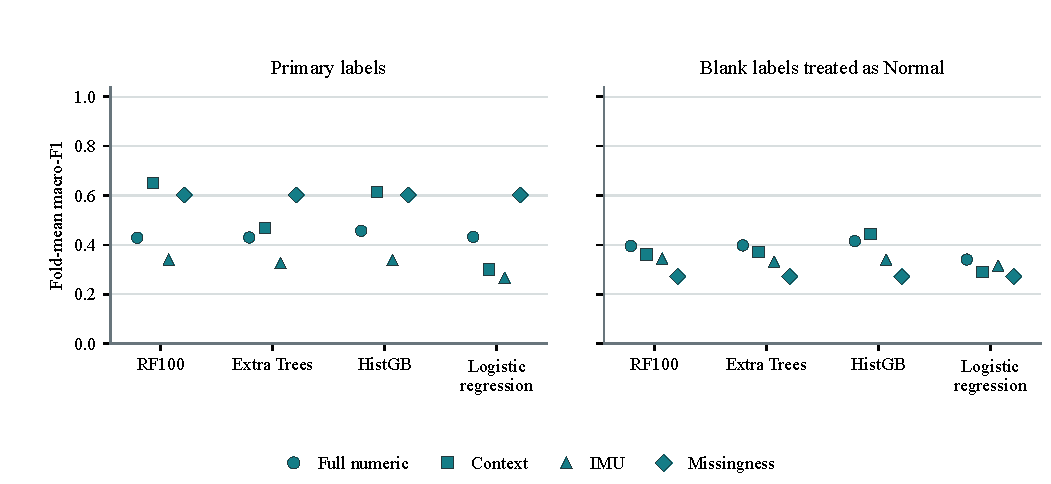
\includegraphics[width=0.99\linewidth]{figures/supp_s1_publication.pdf}
\caption{Recording-heldout feature comparisons for four model families. Points show fold-mean macro-F1; features are associations, not causal effects.}
\end{figure}
\clearpage
\begin{center}
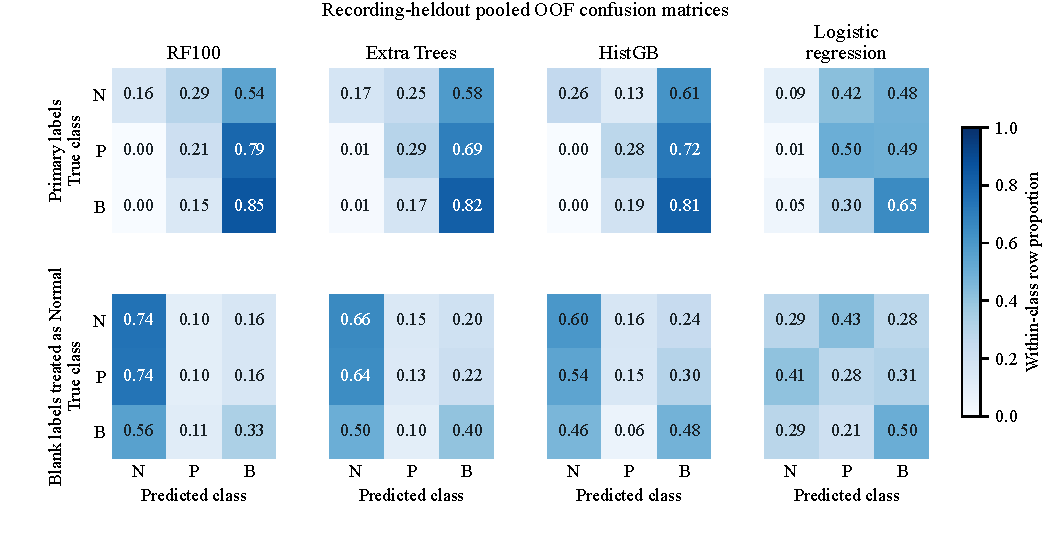
\includegraphics[width=0.99\linewidth]{figures/supp_s2_publication.pdf}
\captionof{figure}{Full-feature recording-heldout pooled confusion matrices, normalized within true class. Diagonal entries are recall. N=Normal, P=Pothole, B=Bump.}
\end{center}
\clearpage
\begin{center}
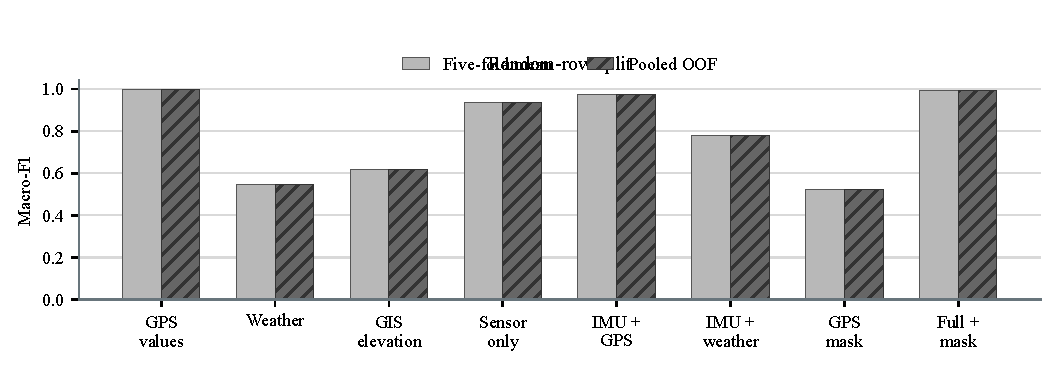
\includegraphics[width=0.99\linewidth]{figures/supp_s3_primary_random.pdf}
\captionof*{figure}{\textbf{Figure S3a.} RF feature ablations under the primary label policy, random-row split. Bars compare five-fold mean and pooled OOF macro-F1.}
\end{center}
\clearpage
\begin{center}
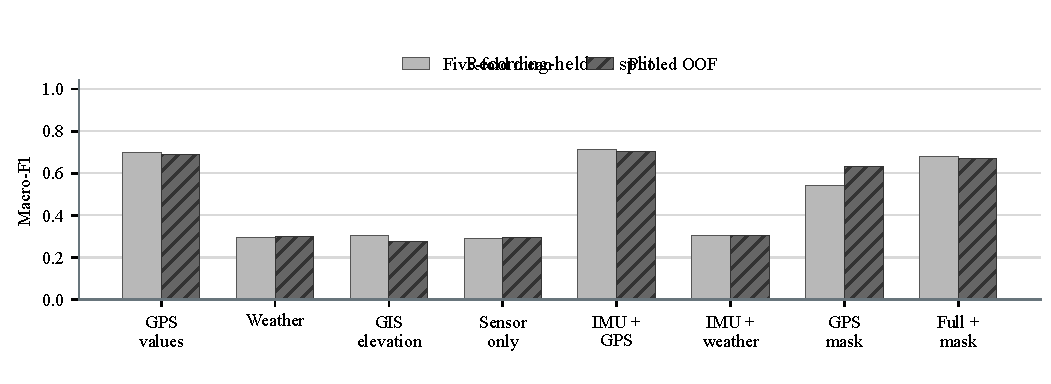
\includegraphics[width=0.99\linewidth]{figures/supp_s3_primary_recording.pdf}
\captionof*{figure}{\textbf{Figure S3b.} RF feature ablations under the primary label policy, recording-heldout split. Bars compare five-fold mean and pooled OOF macro-F1.}
\end{center}
\clearpage
\begin{center}
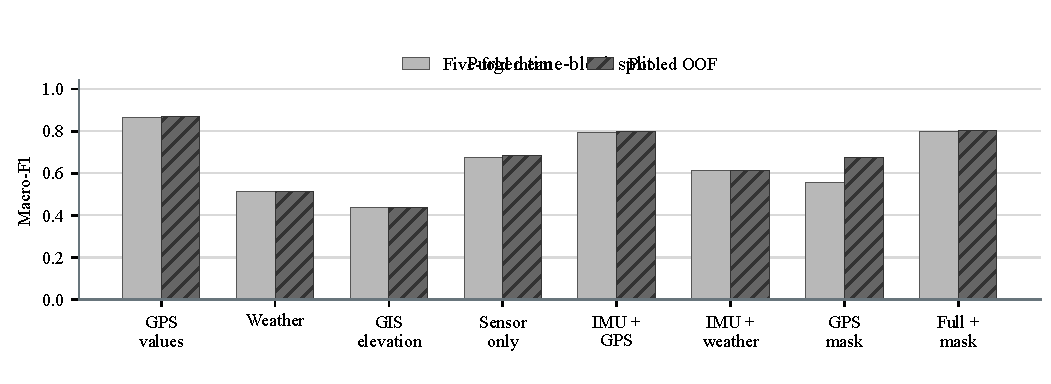
\includegraphics[width=0.99\linewidth]{figures/supp_s3_primary_timeblock.pdf}
\captionof*{figure}{\textbf{Figure S3c.} RF feature ablations under the primary label policy, purged time-block split. Bars compare five-fold mean and pooled OOF macro-F1.}
\end{center}
\clearpage
\begin{center}
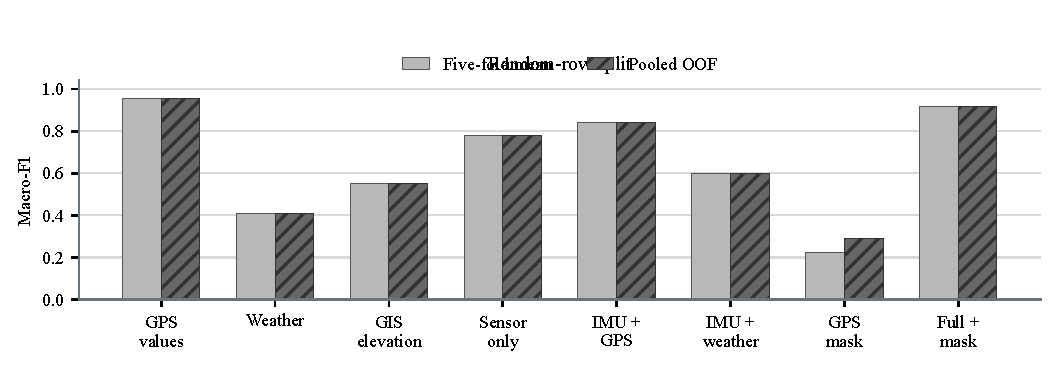
\includegraphics[width=0.99\linewidth]{figures/supp_s3_sensitivity_random.pdf}
\captionof*{figure}{\textbf{Figure S3d.} RF feature ablations under the blank-as-normal sensitivity policy, random-row split. Bars compare five-fold mean and pooled OOF macro-F1.}
\end{center}
\clearpage
\begin{center}
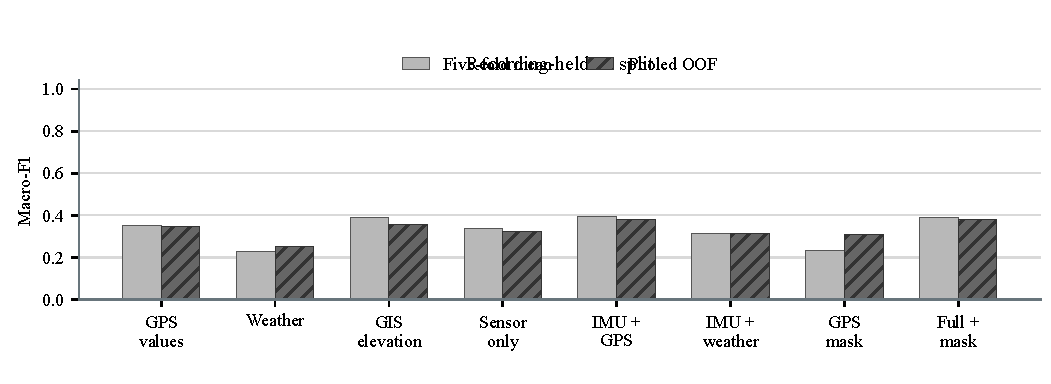
\includegraphics[width=0.99\linewidth]{figures/supp_s3_sensitivity_recording.pdf}
\captionof*{figure}{\textbf{Figure S3e.} RF feature ablations under the blank-as-normal sensitivity policy, recording-heldout split. Bars compare five-fold mean and pooled OOF macro-F1.}
\end{center}
\clearpage
\begin{center}
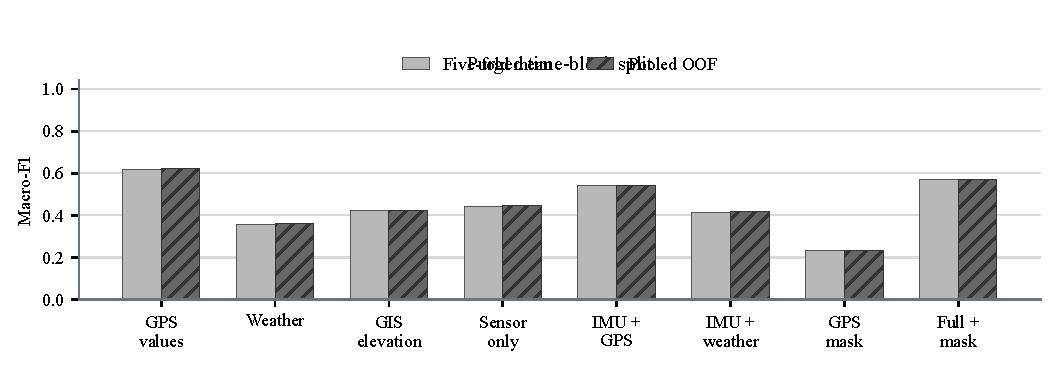
\includegraphics[width=0.99\linewidth]{figures/supp_s3_sensitivity_timeblock.pdf}
\captionof*{figure}{\textbf{Figure S3f.} RF feature ablations under the blank-as-normal sensitivity policy, purged time-block split. Bars compare five-fold mean and pooled OOF macro-F1.}
\end{center}

\clearpage\setcounter{table}{23}
\section*{S13. Common-budget PVS diagnostic}
The diagnostic was fixed after inspecting prior outcomes. It adds 264 computational fits, giving 2,550 total fits including 840 PVS fits, but still only nine PVS acquisitions. V denotes vehicle/driver and S denotes scenario in the axis column; model suffix S denotes inertial sensor features and C adds coordinates and speed. Bias is outer minus inner F1. The two outer targets use different training sizes.
\par\noindent\begin{minipage}{\linewidth}\centering
\captionof{table}{Common per-class training budgets by outer domain.}
\label{tab:s24}
\begin{tabular}{@{}l l r r@{}}
\toprule Axis & Held-out domain & Class 0 & Class 1 \\
\midrule
Vehicle & 1 & 3383 & 53 \\
Vehicle & 2 & 3383 & 53 \\
Vehicle & 3 & 3568 & 56 \\
Scenario & 1 & 2917 & 18 \\
Scenario & 2 & 2917 & 18 \\
Scenario & 3 & 3763 & 57 \\
\bottomrule\end{tabular}\end{minipage}\par\medskip

\par\noindent\begin{minipage}{\linewidth}\begingroup\small\setlength{\tabcolsep}{3pt}
\captionof{table}{Common-budget selected-system domain outcomes.}\label{tab:s25}
\begin{center}\begin{tabular}{@{}l l l l r r r r@{}}
\toprule Axis & ID & Selector & Model & Inner F1 & Outer F1 & Bias & Abs. error \\ \midrule
V & 1 & Random & HGB/S+C & 0.8684 & 0.8444 & -0.0239 & 0.0239 \\
V & 1 & Trip & HGB/S+C & 0.8644 & 0.8444 & -0.0200 & 0.0200 \\
V & 1 & Matched & HGB/S & 0.8383 & 0.8618 & +0.0236 & 0.0236 \\
V & 2 & Random & HGB/S+C & 0.8549 & 0.8590 & +0.0041 & 0.0041 \\
V & 2 & Trip & HGB/S+C & 0.8166 & 0.8590 & +0.0425 & 0.0425 \\
V & 2 & Matched & HGB/S+C & 0.8069 & 0.8590 & +0.0521 & 0.0521 \\
V & 3 & Random & HGB/S+C & 0.8510 & 0.8371 & -0.0139 & 0.0139 \\
V & 3 & Trip & HGB/S+C & 0.8398 & 0.8371 & -0.0027 & 0.0027 \\
V & 3 & Matched & HGB/S+C & 0.8415 & 0.8371 & -0.0044 & 0.0044 \\
S & 1 & Random & HGB/S+C & 0.8960 & 0.6873 & -0.2087 & 0.2087 \\
S & 1 & Trip & RF/S+C & 0.8919 & 0.7048 & -0.1872 & 0.1872 \\
S & 1 & Matched & HGB/S & 0.8501 & 0.6842 & -0.1659 & 0.1659 \\
S & 2 & Random & HGB/S+C & 0.8365 & 0.5588 & -0.2777 & 0.2777 \\
S & 2 & Trip & HGB/S+C & 0.7730 & 0.5588 & -0.2142 & 0.2142 \\
S & 2 & Matched & HGB/S & 0.7557 & 0.5447 & -0.2110 & 0.2110 \\
S & 3 & Random & HGB/S+C & 0.8770 & 0.8787 & +0.0017 & 0.0017 \\
S & 3 & Trip & HGB/S+C & 0.8517 & 0.8787 & +0.0270 & 0.0270 \\
S & 3 & Matched & HGB/S & 0.7163 & 0.8565 & +0.1402 & 0.1402 \\
\bottomrule\end{tabular}\end{center}\endgroup\end{minipage}\par\medskip

\par\noindent\begin{minipage}{\linewidth}\begingroup\small\setlength{\tabcolsep}{3pt}
\captionof{table}{Historical-full-budget selected-system domain outcomes.}\label{tab:s26}
\begin{center}\begin{tabular}{@{}l l l l r r r r@{}}
\toprule Axis & ID & Selector & Model & Inner F1 & Outer F1 & Bias & Abs. error \\ \midrule
V & 1 & Random & HGB/S+C & 0.8684 & 0.8129 & -0.0554 & 0.0554 \\
V & 1 & Trip & HGB/S+C & 0.8644 & 0.8129 & -0.0515 & 0.0515 \\
V & 1 & Matched & HGB/S & 0.8383 & 0.8241 & -0.0142 & 0.0142 \\
V & 2 & Random & HGB/S+C & 0.8549 & 0.9004 & +0.0455 & 0.0455 \\
V & 2 & Trip & HGB/S+C & 0.8166 & 0.9004 & +0.0838 & 0.0838 \\
V & 2 & Matched & HGB/S+C & 0.8069 & 0.9004 & +0.0935 & 0.0935 \\
V & 3 & Random & HGB/S+C & 0.8510 & 0.8320 & -0.0190 & 0.0190 \\
V & 3 & Trip & HGB/S+C & 0.8398 & 0.8320 & -0.0077 & 0.0077 \\
V & 3 & Matched & HGB/S+C & 0.8415 & 0.8320 & -0.0094 & 0.0094 \\
S & 1 & Random & HGB/S+C & 0.8960 & 0.7046 & -0.1914 & 0.1914 \\
S & 1 & Trip & RF/S+C & 0.8919 & 0.7280 & -0.1640 & 0.1640 \\
S & 1 & Matched & HGB/S & 0.8501 & 0.6949 & -0.1552 & 0.1552 \\
S & 2 & Random & HGB/S+C & 0.8365 & 0.7800 & -0.0566 & 0.0566 \\
S & 2 & Trip & HGB/S+C & 0.7730 & 0.7800 & +0.0069 & 0.0069 \\
S & 2 & Matched & HGB/S & 0.7557 & 0.8688 & +0.1131 & 0.1131 \\
S & 3 & Random & HGB/S+C & 0.8770 & 0.9113 & +0.0342 & 0.0342 \\
S & 3 & Trip & HGB/S+C & 0.8517 & 0.9113 & +0.0596 & 0.0596 \\
S & 3 & Matched & HGB/S & 0.7163 & 0.8865 & +0.1702 & 0.1702 \\
\bottomrule\end{tabular}\end{center}\endgroup\end{minipage}\par\medskip

\subsection*{S13.1. Prospective acquisition and confirmation plan}
Further evidence should come from genuinely new acquisitions across dates, route families, vehicles, and drivers, or from another independently collected event-labelled dataset with authentic acquisition identifiers. Repeated passes and physical anomalies should retain shared route and event identities. Driver and vehicle identities should be crossed where feasible. Develop any revised method, thresholds, and primary metrics on a development cohort, then freeze them before evaluation on untouched whole acquisitions. Existing PVS outer results have been inspected and cannot provide confirmation. Acquisition counts must be planned using expected effects and desired uncertainty at the acquisition or route-family level. No fixed window or fit count guarantees adequacy. The earlier dataset-search screening alone was a logistics note; the subsequently executed Mexico/Puebla subset evaluation is reported separately in S14 and does not confirm an improved method.

\section*{S14. Mexico/Puebla released-subset replication}
This is an additional-source exploratory evaluation audit, not preregistration or confirmation of an improved algorithm. Source arrays, label distributions and readiness were examined before the predictive protocol was frozen. The source is the Applied Sciences publisher supplement \cite{mexico2025}; the related Vehicles article describes the two-route outbound/return organization \cite{mexico2026}. These publications are not counted as two independent collections. The archive's four JSON arrays contain 36,000 source positions; the reported complete population exceeds 360,000. The subset/version mapping remains unresolved. No signal statistic authenticates field provenance. No misconduct inference follows from this discrepancy or the fixed label durations.

The four source SHA256 identities, complete raw-array audit, retained infeasible v1 protocol, v 2 protocol, code and exact indices are packaged as compact evidence. No exact six-channel row or consecutive 2/5/10/25-position fragment is shared across different files; all values are finite. The six sensor channels include vibration described as derived from acceleration, so only acceleration x/y/z is used. Event annotation runs are always 6 positions (pothole) or 11(bump/braking). The first 50-position proposal retained no target events and was abandoned before any fitting. V2 fixes 10-position nonoverlapping windows at starts 0,10,...,8990 per source. Exclude any window containing braking; otherwise retain the unique literal majority only at count 6 or more. Blank=0(non-event), pothole=1, bump=2. This release non-event is not a claim that all such physical roads are normal.

\begin{minipage}{\linewidth}\begingroup\small
\captionof{table}{Retained nonoverlap window counts; source files have 9,000 positions each.}\label{tab:s27}
\begin{tabularx}{\linewidth}{Xrrrr}\toprule
Source & Non-event & Pothole & Bump & Total\\\midrule
Trip 1 &454&48&96&598\\
Trip 2 &444&64&93&601\\
Trip 3 &484&67&80&631\\
Trip 4 &516&78&80&674\\\midrule
Total &1,898&257&349&2,504\\\bottomrule
\end{tabularx}\endgroup\end{minipage}

Outer folds hold out trips 1+2(urban) or 3+4(suburban), respectively. These route identities derive from source documentation and are not verified from released GPS. The two inner selectors are stratified random two-fold (seed 42) and leave-one-whole-trip two-fold within the single development route. A nested route-matched selector cannot be estimated here. Training is sampled without replacement to the minimum count of each class across the four inner training pools, preserving class imbalance. Budgets (no-event, pothole, bump) are (484,67,80) when holding out urban and (444,48,93) when holding out suburban. Full refits use all 1,305 or 1,199 development windows; common-budget refits use the corresponding 631 or 585 windows. The targets are reported separately. Random subsampling also changes class/row composition and does not isolate a causal sample-size effect. Exact saved memberships, rather than seed-only regeneration, are authoritative.

Each window has 36 features: mean, population SD, min, max, RMS, 25th/50th/75th percentiles and first-difference population SD for x, y, z and vector magnitude. Median imputation is fitted on actual training rows. RF uses 100 trees, depth 20, leaf minimum 5, sqrt feature sampling and balanced class weights. HGB uses 100 iterations, 31 leaves, learning rate 0.1, L2=1, balanced class weights and no early stopping. Both use seed 42; no tuning or candidate additions occur. Each selector chooses the larger pooled OOF three-class macro-F1, with RF first on exact ties. Selection is saved before outer evaluation; both selectors share the same candidate-specific outer refits. The 24 fits comprise 16 inner and 8 outer fits. All models/predictions are preserved in the workspace; the manuscript package omits raw signals and model binaries.

\begin{minipage}{\linewidth}\begingroup\small
\captionof{table}{Mexico task: primary full-development refit.}\label{tab:s28}
\renewcommand{\arraystretch}{1.2}
\begin{tabularx}{\linewidth}{lXlrrr}
\toprule
Held-out route & Inner selector & Chosen & Inner F1 & Outer F1 & Abs. error \\
\midrule
Urban (1+2) & Random & RF & 0.9922 & 0.9934 & 0.0012 \\
Urban (1+2) & Whole-trip & RF & 0.9922 & 0.9934 & 0.0012 \\
\midrule
Suburban (3+4) & Random & RF & 0.9934 & 0.9960 & 0.0026 \\
Suburban (3+4) & Whole-trip & RF & 0.9950 & 0.9960 & 0.0010 \\
\bottomrule\end{tabularx}
\par\smallskip\footnotesize F1 is macro-F1 on three fixed classes (higher is better); absolute estimation error is lower-is-better. There are two documentation-derived route families, with no population confidence interval. Both selectors share each selected outer model.\endgroup\end{minipage}


\begin{minipage}{\linewidth}\begingroup\small
\captionof{table}{Mexico task: separately specified common-budget outer sensitivity.}\label{tab:s29}
\renewcommand{\arraystretch}{1.2}
\begin{tabularx}{\linewidth}{lXlrrr}
\toprule
Held-out route & Inner selector & Chosen & Inner F1 & Outer F1 & Abs. error \\
\midrule
Urban (1+2) & Random & RF & 0.9922 & 0.9918 & 0.0004 \\
Urban (1+2) & Whole-trip & RF & 0.9922 & 0.9918 & 0.0004 \\
\midrule
Suburban (3+4) & Random & RF & 0.9934 & 0.9960 & 0.0026 \\
Suburban (3+4) & Whole-trip & RF & 0.9950 & 0.9960 & 0.0010 \\
\bottomrule\end{tabularx}
\par\smallskip\footnotesize F1 is macro-F1 on three fixed classes (higher is better); absolute estimation error is lower-is-better. There are two documentation-derived route families, with no population confidence interval. Both selectors share each selected outer model.\endgroup\end{minipage}


The mean whole-trip-minus-random selected outer-F1 difference is exactly 0 under both targets. Mean absolute-error differences are -0.0008369747 (full) and -0.0007920153 (common budget); these are descriptive means of two route-specific pairs, not population effects. No bootstrap interval, p-value, or improvement threshold is applied. Small errors and identical selections are retained as an additional-source counterexample, not hidden because they do not reproduce PVS. Blank semantics, short windows, processed-subset provenance and only two documented route families restrict comparison with the larger RoadSens/PVS tasks. No RoadSens-trained model is transferred to Mexico.

Independent reconstruction checks all 3,600 raw-window inclusion decisions, 2,504 included label/feature records, all exact split and per-class-budget memberships, 24 model byte hashes and reloaded predictions, training imputation medians, fixed parameters, all confusion/per-class metrics, pooled candidate selection and both paired summaries. The verification code does not import the execution script or refit models. Raw reconstruction matches features within 1e-10; prediction replay uses the frozen feature values. The frozen protocol and execution SHA256 identities, preflight checksum and result hash are supplied with the evidence.

\subsection*{S14.1. Indonesia source expansion: label versions require clarification}
The complete author repository ZIP linked to the Indonesia study \cite{indonesia2021} was obtained on 26 October 2026 and contains 60 CSV files, including concurrent phone streams, chunks and alternate exports. Readiness inspection identified six motorcycle session families and ten timestamped car-session candidates; these counts are not independent roads or necessarily complete field acquisitions. No classifier was fitted. The five base motorcycle CSVs overlap wider six-class exports and do not add acquisition units. Crucially, matching exact first 20 fields of Samsung records shows original labels agree with wider column 21 on 20,782/25,833 matched rows in M5-1 and 4,456/5,206 in M5-4. Wider column 22 also differs (22,558/25,833 and 4,693/5,206). New class codes and processed/LSTM-export fields are not documented by the base README. These wider labels are not silently accepted as ground truth. The row comparisons and source hashes are retained. Label-version clarification is required before a wider-source evaluation; mere availability of more files is insufficient. Repeated passes and overlapping road geography must remain grouped.



\begin{thebibliography}{9}
\bibitem{roadsens} A. Khandakar, D. G. Michelson, S. G. Rabbani, F. B. Shafi, M. F. Ahamed, K. R. Rahman, M. A. Rahman, M. F. Nabi, M. A. Ayari, K. Khan, and P. N. Suganthan, ``RoadSens-4M: A Multimodal Smartphone \& Camera Dataset for Holistic Road-way Analysis,'' \emph{Scientific Data}, vol. 13, Art. no. 1036, 2026. doi: \href{https://doi.org/10.1038/s41597-026-07072-y}{10.1038/s41597-026-07072-y}. Code: \url{https://github.com/rabbanishaikh/One-Million-Observations-Dataset}.
\bibitem{roadsensdata} A. Khandakar et al., ``RoadSens-4M Dataset,'' Figshare, version 3, 2025 [repository citation year; v3 publication-date field: 24 February 2026]. doi: \href{https://doi.org/10.6084/m9.figshare.30341143.v3}{10.6084/m9.figshare.30341143.v3}. CC BY 4.0.
\bibitem{ckdppinnfed} A. Khandakar, D. G. Michelson, M. M. Mia, G. M. A. Sakeef, K. Khan, and M. A. Ayari, ``CKDP-PINNFed: Dual-Layer Privacy Framework Combining Contextual K-Anonymity and Differential Privacy with Physics-Informed Federated Learning for Explainable Crowdsourced Road Anomaly Detection,'' \emph{Green Energy and Intelligent Transportation}, Art. no. 100433, 2026. doi: \href{https://doi.org/10.1016/j.geits.2026.100433}{10.1016/j.geits.2026.100433}.
\bibitem{roberts} D. R. Roberts, V. Bahn, S. Ciuti, M. S. Boyce, J. Elith, G. Guillera-Arroita, S. Hauenstein, J. J. Lahoz-Monfort, B. Schr\"oder, W. Thuiller, D. I. Warton, B. A. Wintle, F. Hartig, and C. F. Dormann, ``Cross-validation strategies for data with temporal, spatial, hierarchical, or phylogenetic structure,'' \emph{Ecography}, vol. 40, no. 8, pp. 913--929, 2017. doi: \href{https://doi.org/10.1111/ecog.02881}{10.1111/ecog.02881}.
\bibitem{ploton} P. Ploton, F. Mortier, M. R\'ejou-M\'echain, N. Barbier, N. Picard, V. Rossi, C. F. Dormann, G. Cornu, G. Viennois, N. Bayol, A. Lyapustin, S. Gourlet-Fleury, and R. P\'elissier, ``Spatial validation reveals poor predictive performance of large-scale ecological mapping models,'' \emph{Nature Communications}, vol. 11, Art. no. 4540, 2020. doi: \href{https://doi.org/10.1038/s41467-020-18321-y}{10.1038/s41467-020-18321-y}.
\bibitem{stride} A. Khandakar et al., ``STRIDE (Sensor Technologies for Road Insights and Driving Evaluation) Dataset,'' Figshare, version 4, 2024. doi: \href{https://doi.org/10.6084/m9.figshare.25460755.v4}{10.6084/m9.figshare.25460755.v4}. CC BY 4.0.
\bibitem{stridepaper} A. Khandakar, D. G. Michelson, M. Naznine, A. Salam, M. Nahiduzzaman, K. M. Khan, P. N. Suganthan, M. A. Ayari, H. Menouar, and J. Haider, ``Harnessing Smartphone Sensors for Enhanced Road Safety: A Comprehensive Dataset and Review,'' \emph{Scientific Data}, vol. 12, Art. no. 418, 2025. doi: \href{https://doi.org/10.1038/s41597-024-04193-0}{10.1038/s41597-024-04193-0}.
\bibitem{pvsdata} J. Menegazzo and A. von Wangenheim, ``Passive Vehicular Sensors (PVS) datasets,'' official repository-linked release. \url{https://www.kaggle.com/datasets/jefmenegazzo/pvs-passive-vehicular-sensors-datasets}. Accessed 17 October 2026. CC BY-NC-ND 4.0.
\bibitem{pvspaper} J. Menegazzo and A. von Wangenheim, ``Speed Bump Detection Through Inertial Sensors and Deep Learning in a Multi-contextual Analysis,'' \emph{SN Computer Science}, vol. 4, Art. no. 18, 2023 [online 17 October 2022]. doi: \href{https://doi.org/10.1007/s42979-022-01438-w}{10.1007/s42979-022-01438-w}.
\bibitem{mexico2025} A. Aguilar-Gonz\'alez and A. Medina Santiago, ``CNN-Based Road Event Detection Using Multiaxial Vibration and Acceleration Signals,'' \emph{Applied Sciences}, vol.15, no.18, Art.10203, 2025. doi: \href{https://doi.org/10.3390/app151810203}{10.3390/app151810203}. Publisher supplementary archive accessed 26 October 2026.
\bibitem{mexico2026} A. Aguilar-Gonz\'alez and A. Medina Santiago, ``Context-Aware Road Event Detection Using Hybrid CNN--BiLSTM Networks,'' \emph{Vehicles}, vol.8, no.1, Art.4, 2026. doi: \href{https://doi.org/10.3390/vehicles8010004}{10.3390/vehicles8010004}.
\bibitem{indonesia2021} B. D. Setiawan et al., `A Machine Learning Framework for Balancing Training Sets of Sensor Sequential Data Streams, \emph{Sensors}, vol.21, no.20, Art.6892, 2021. doi: \href{https://doi.org/10.3390/s21206892}{10.3390/s21206892}. Data: \url{https://github.com/s-budidarma/dataset-smarphone-sensor-for-road-surface-monitoring}.
\end{thebibliography}
